\chapter{Auswertung}
\label{cha:Auswertung}

\section{Bestimmung des Erdmagnetfeldes}
\label{sec:erdmagnetfeld}
Zu Beginn wird, wie im Kapitel \ref{cha:Durchführung} erklärkt, die vertikal Komponente des Erdmagnetfeldes kompensiert. Dies geschieht mit einem entgegengerichtetem Magnetfeld. 
Dieses wird so eingestellt, dass der Peak bei $B = 0$ möglichst dünn wird. Anhand von Optimierung kann dann das Kompensationsmagnetfeld gemessen werden. Dieses ist betragsmäßig
gleich dem Erdmagnetfeld. Dadruch wurde das Erdmagnetfeld zu $B_\mathrm{Erde} = \qty{34.94}{\micro\tesla}$ bestimmt. 

\section{Bestimmung der $g$-Faktoren und der Kernspins}
\label{sec:kernspin}
Danach wurden die Spulen verwendet. Dabei handelt es sich um zwei seperate Helmholtz-Spulen, wovon eine als konstantes Feld verwendet wurde und die andere zum sweepen. 
Aufgrund der identischen Richtung der Felder können diese durch Superposition addiert werden. Das Magnetfeld einer Helmholtzspule ist dabei gegeben durch
\begin{equation}
    \label{eqn:helmholtz}
    B = \mu_0\frac{8NI}{\sqrt{125}R}\,.
\end{equation}
In dieser Gleichung ist $N$ die Windugszahl einer Spule, $I$ der treibende Strom und $R$ der Widerstand der Spulen. 
Gleichung \eqref{eqn:g_formel} zeigt einen linearen Zusammenhang zwischen Frequenz des angelegten HF-Feldes und dem $B$-Feld. Daher kann ein Ansatz über eine Polynom ersten Grades 
durchgeführt werden.
\begin{equation*}
    B = \frac{h}{g_F\mu_B}f + b = af + b 
\end{equation*}
Der konstante Faktor wird in diesem Fall variabel gelassen um statistische Fehler zu minimieren. Der $g$-Faktor steckt in der Steigung der Gleichung. Aus einem linearen Fit der Messwerte 
von $B$ und $f$ kann dieser dann bestimmt werden. Die Messwerte mit den Ausgleichsgeraden sind in Abbildung \ref{fig:Messung} dargestellt.

\begin{figure}
    \centering
    \includegraphics[width = \textwidth]{build/regression.pdf}
    \caption{Messdaten mit durchgeführter Regression.}
    \label{fig:Messung}
\end{figure}

Der Fit hat die folgenden zwei Sätze an Parameter ergeben, jeweils für den Peak eines Rubidium-Isotops.
\begin{align*}
    a_1 &=  \qty{1.453(0.005)e-10}{\tesla\per\hertz} \; b_1 &=  \qty{2.433(0.030)e-05}{\tesla}\\
    a_2 &=  \qty{2.177(0.006)e-10}{\tesla\per\hertz} \; b_2 &=  \qty{2.406(0.035)e-05}{\tesla}\\
\end{align*}

Durch diese Parameter ergeben sich die $g$-Faktoren 
\begin{align*}
    g_{F,1} &=  \num{0.4917(0.0016)}\\
    g_{F,2} &=  \num{0.3282(0.0009)}.
\end{align*}

Mit diesen Werten und den Quantenzahlen für Rubidium kann gemäß Gleichung \eqref{eqn:g_F} der Kernspin berechnet werden. 
Daraus folgen die Werte
\begin{align*}
    I_{1} &= \num{1.534(0.007)}\\
    I_{2} &= \num{2.547(0.008)}.
\end{align*}
Daher muss der erste Peak zum \ce{^{87}_{37}Rb} gehören und der zweite zu \ce{^{85}_{37}Rb}.

\section{Isotopenverhältnis}
\label{sec:isotop}
Da nun ermittelt wurde, welcher Peak zu welchem Isotop gehört kann über das Verhältnis der Amplitude der Peaks das Isotopenverhältnis bestimmt werden, da die Amplitude direkt von der 
Anzahl der Atome abhängt. Dazu wurde die Aufnahme eines Oszilloskops ausgewertet. Dieses Bild ist in Abbildung \ref{fig:isotop} gezeigt.

\begin{figure}
    \centering
    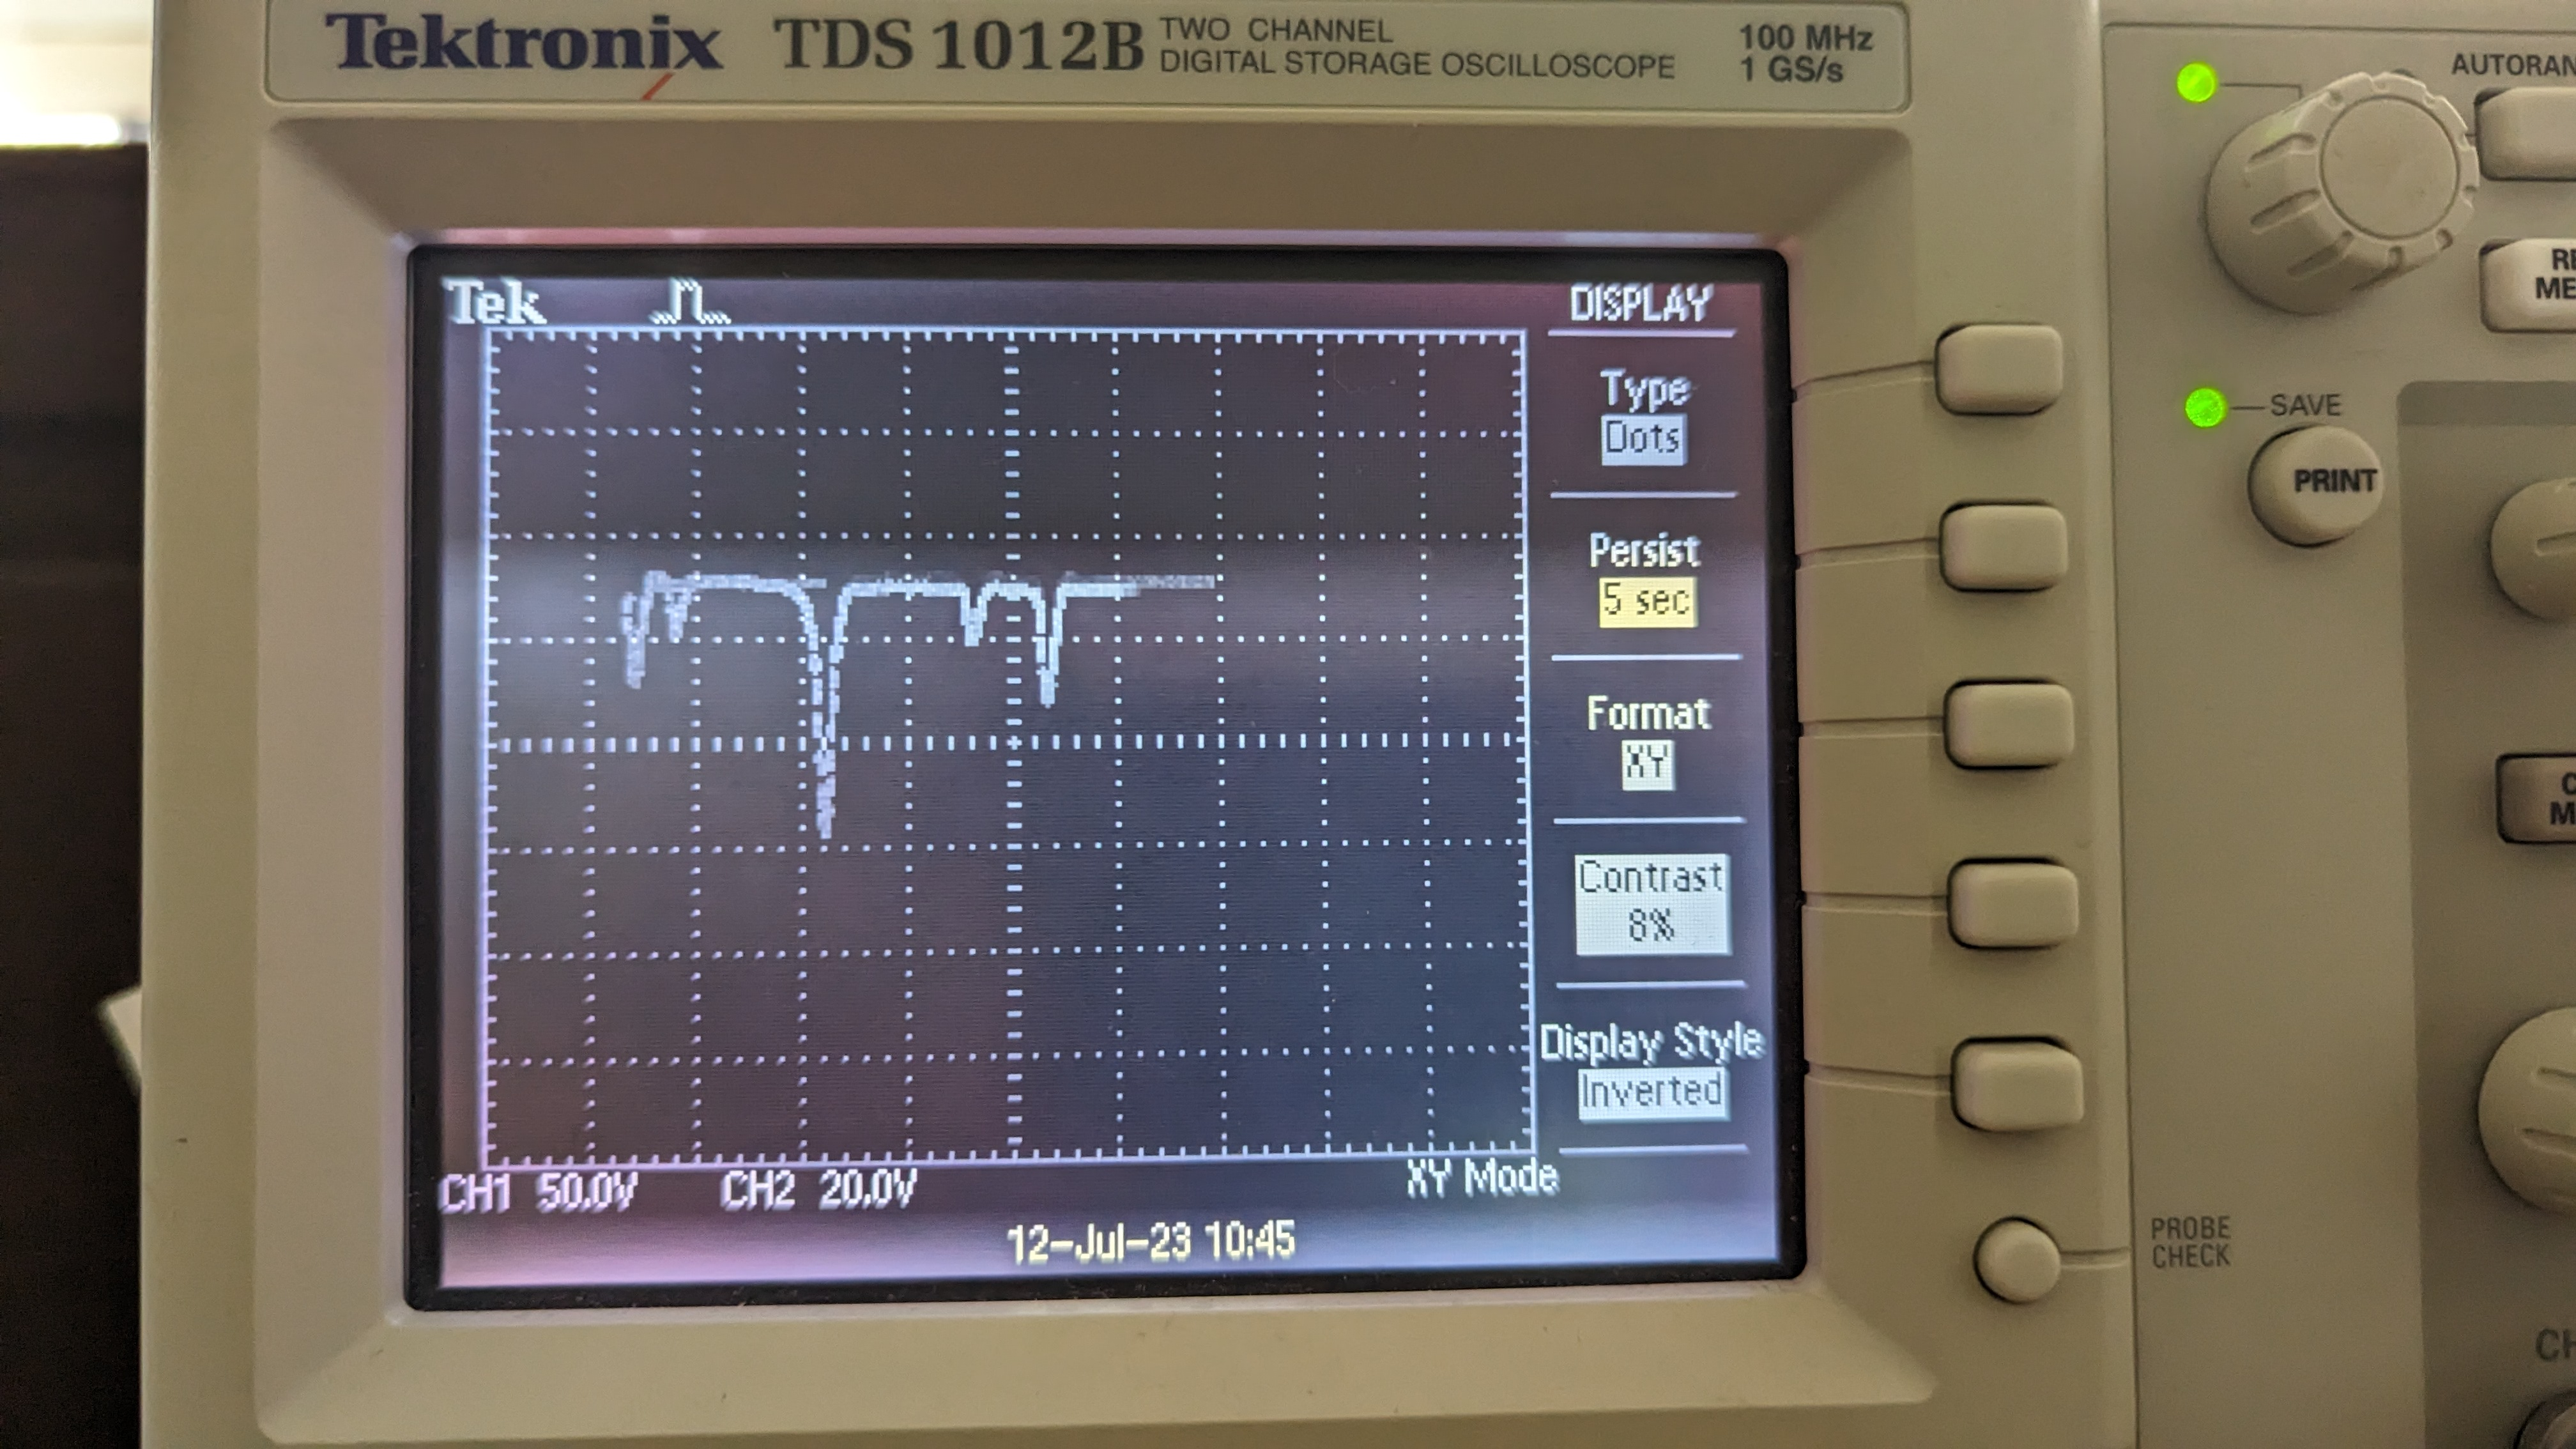
\includegraphics[width = \textwidth]{content/v21_bilder/isotop.jpg}
    \caption{Bild des Oszilloskops bei einer Messung bei $f_{\mathrm{HF}} = \qty{100}{\kilo\hertz}$.}
    \label{fig:isotop}
\end{figure}

Die Amplituden wurde zu $\qty{6.2}{\centi\metre}$ und $\qty{12.6}{\centi\metre}$ bestimmt. Daraus ergibt sich ein Isotopenverhältnis von 
\begin{equation}
    \label{eqn:isotopen}
    \frac{^{85}\symup{Rb}}{^{87}\symup{Rb}} \approx \num{0.49}\,.
\end{equation}
